\documentclass[11pt, oneside]{article}   	% use "amsart" instead of "article" for AMSLaTeX format
\usepackage{geometry}                		% See geometry.pdf to learn the layout options. There are lots.
\geometry{letterpaper}                   		% ... or a4paper or a5paper or ... 
\usepackage{graphicx}				% Use pdf, png, jpg, or eps§ with pdflatex; use eps in DVI mode
								% TeX will automatically convert eps --> pdf in pdflatex		
\usepackage{amssymb}
\usepackage{amsmath}
\usepackage{parskip}
\usepackage{color}
\usepackage{hyperref}

\graphicspath{{/Users/telliott_admin/Dropbox/Tex/png/}}
% \begin{center} \includegraphics [scale=0.4] {gauss3.png} \end{center}

%break
\title{Vector cross product}
\date{}

\begin{document}
\maketitle
\Large
\label{sec:Vector_cross_product}

Suppose we have two ordinary vectors $\mathbf{u}$ and $\mathbf{v}$.  These must be in $\mathbb{R}3$ because the cross-product is only defined for vectors in $\mathbb{R}3$.

Their respective lengths are $u$ and $v$.

We write the cross-product as
\[ \mathbf{u} \times \mathbf{v} = \mathbf{w}  \]
The simplest definition is that the magnitude of $\mathbf{w}$ is 
\[ w = uv \ \sin \theta \]

The symmetry with the dot product is obvious.  Also
\[ | \mathbf{u} \times \mathbf{v} |^2 + | \mathbf{u} \cdot \mathbf{v} |^2 = (uv)^2 \]

The direction is defined by saying that $\mathbf{w}$ is orthogonal to the plane which contains both $\mathbf{u}$ and $\mathbf{v}$, and its sign is given by the right-hand rule.  Curl the fingers of your right hand around in the direction from $\mathbf{u}$ to $\mathbf{v}$.  Your thumb points in the same direction as $\mathbf{w}$.  

The term $\sin \theta$ means that the cross-product of any vector with itself is zero.
\[ \mathbf{a} \times \mathbf{a} = \mathbf{0}  \]

To make the notation simpler, we define
\[ \mathbf{u} = \langle p,q,r \rangle \]
\[ \mathbf{v} = \langle x,y,z \rangle \]
and in order to compute the cross product, we form what looks like a really weird matrix
\[
\begin{bmatrix} 
  \hat{\mathbf{i}}  & \hat{\mathbf{j}}  &  \hat{\mathbf{k}} \\ 
  p  &  q & r \\
  x  &  y & z
\end{bmatrix}
\]
and write its "determinant"
\[ \mathbf{u} \times \mathbf{v}  = (qz - ry) \ \hat{\mathbf{i}} + (rx - pz) \  \hat{\mathbf{j}}  + (py - qx) \ \hat{\mathbf{k}}  \]
We can show that the resulting vector is orthogonal to the two starting vectors, $\mathbf{u}$ and $\mathbf{v}$.  Test that by forming the dot product with $\mathbf{u}$.
\[ \mathbf{u} \cdot (\mathbf{u} \times \mathbf{v})  =  p(qz - ry) + q(rx - pz)   + r(py - qx)  \] 
The first and fourth terms cancel, the second and fifth terms cancel, and the third and sixth terms also cancel.  

So $\mathbf{u} \cdot (\mathbf{u} \times \mathbf{v}) = 0$, and $\mathbf{v} \cdot (\mathbf{u} \times \mathbf{v}) = 0$ as well.  

In fact, a very common use for the cross-product is to find the normal vector to a plane in vector calculus.

As an aside, we could have skipped this calculation.  The following rule holds for vectors:
\[ \mathbf{a} \cdot ( \mathbf{b} \times \mathbf{c} ) = ( \mathbf{a} \times \mathbf{b} ) \cdot \mathbf{c} \]
(we will explore triple products below).
So
\[ \mathbf{u} \cdot (\mathbf{u} \times \mathbf{v}) = (\mathbf{u} \times \mathbf{u}) \cdot \mathbf{v} = 0 \]
\[ \mathbf{v} \cdot (\mathbf{u} \times \mathbf{v}) = - \mathbf{v} \cdot (\mathbf{v} \times \mathbf{u}) = - (\mathbf{v} \times \mathbf{v}) \cdot \mathbf{u}) = 0 \]

\subsection*{About the angle}

How to show that

\[ \mathbf{a} \times \mathbf{b} = |\mathbf{a}| |\mathbf{b}| \sin \theta \ \hat{\mathbf{n}}  \]

where $\hat{\mathbf{n}}$ is perpendicular to $\mathbf{a}$ and $\mathbf{b}$.

\[ |\mathbf{a} \times \mathbf{b} | = |\mathbf{a}| |\mathbf{b}| \sin \theta \]

According to wikipedia, this is the \emph{definition} of the cross-product, and from this one can derive the expression that we got by setting up our matrix and computing its "determinant."  So that is what we are going to do.

I am going to go back to the notation we had before, rather than use subscripts like $a_x$, etc.

\[ \mathbf{u} = \langle p,q,r \rangle \]
\[ \mathbf{v} = \langle x,y,z \rangle \]

We proceed from the "determinant" definition of the cross product and show that the length of that vector squared plus the square of the dot product is equal to $u^2v^2$.  By the argument we made above, the magnitude of the cross product is then equal to $uv \sin \theta$.

\[ \mathbf{u} \times \mathbf{v}  = (qz-ry) \hat{\mathbf{i}}  + (rx-pz) \hat{\mathbf{j}} + (py-qx) \hat{\mathbf{k}}\]

\[ |\mathbf{u} \times \mathbf{v}|^2 = (qz-ry)^2 + (rx-pz)^2 + (py-qx)^2 \]
\[ = (qz)^2 - 2qryz + (ry)^2 + (rx)^2 - 2prxz + (pz)^2 + (py)^2 - 2pqxy + (qx)^2 \]


\[ \mathbf{u} \cdot \mathbf{v} = px + qy + rz \]
\[ (\mathbf{u} \cdot \mathbf{v})^2 = (px)^2 + (qy)^2 + (rz)^2 + 2pqxy + 2prxz + 2qryz \]

When we add these together, all the terms with cofactor $2$ cancel so that leaves

\[ | \mathbf{u} \times \mathbf{v} |^2 + (\mathbf{u} \cdot \mathbf{v})^2 \]
\[ =  (qz)^2 + (ry)^2 + (rx)^2 + (pz)^2 + (py)^2 + (qx)^2 + (px)^2 + (qy)^2 + (rz)^2 \]


rearranging terms
\[ = (px)^2 + (py)^2 + (pz)^2 + (qx)^2 + (qy)^2 + (qz)^2 + (rx)^2 +(ry)^2   + (rz)^2 \]

\[ = (p^2 + q^2 + r^2)(x^2 + y^2 + z^2) \]

\[ = |\mathbf{u}|^2 |\mathbf{v}|^2 \]

That was tedious, but it we made it.

All of these properties of the cross-product are connected.
\[ \mathbf{a}  \cdot (\mathbf{a} \times \mathbf{b}) = \mathbf{b}  \cdot (\mathbf{a} \times \mathbf{b}) = 0 \]
\[ \mathbf{a} \times \mathbf{b} =  \ \langle qu-rt, rs-pu, pt-qs \rangle \]
\[ |\mathbf{a} \times \mathbf{b}|  = |\mathbf{a}| |\mathbf{b}| \sin \theta \]
\[ | \mathbf{a} \times \mathbf{b} |^2 + (\mathbf{a} \cdot \mathbf{b})^2 = |\mathbf{a}|^2 |\mathbf{b}|^2 \]

\subsection*{Triple products}
Suppose we have
\[\mathbf{a} = \ \langle p,q,r \rangle \]
\[\mathbf{b} = \ \langle s,t,u \rangle \]
\[\mathbf{c} = \ \langle x,y,z \rangle \]
And
\[ \mathbf{a} \times \mathbf{b} =  \ \langle qu-rt, rs-pu, pt-qs \rangle \]
\[ \mathbf{b} \times \mathbf{c} =  \ \langle tz-uy, ux-sz, sy-tx \rangle \]
\[ \mathbf{a} \times \mathbf{c} =  \ \langle qz-ry, rx-pz, py-qx \rangle \]
Algebraically
\[ \mathbf{a} \cdot (\mathbf{b} \times \mathbf{c}) = p(tz-uy) + q(ux-sz) + r(sy-tx)  \]
\[ \mathbf{b} \cdot (\mathbf{c} \times \mathbf{a}) = s(ry-qz) + t(pz-rx) + u(qx-py) \]
\[ \mathbf{c} \cdot (\mathbf{a} \times \mathbf{b}) = x(qu-rt) + y(rs-pu) + z(pt-qs) \]
So
\[ \mathbf{a} \cdot (\mathbf{b} \times \mathbf{c}) = \mathbf{b} \cdot (\mathbf{c} \times \mathbf{a}) = \mathbf{c} \cdot (\mathbf{a} \times \mathbf{b}) \]

The way to remember this is that these are all the same cyclic permutation.

A much simpler proof is to remember that the cross-product $\mathbf{a} \times \mathbf{b}$ is the area of the parallelogram formed by $\mathbf{a}$ and $\mathbf{b}$ and the \emph{scalar} triple product is the signed volume of the parallelipiped formed by the three vectors.   Signed meaning that $\mathbf{c} \cdot (\mathbf{a} \times \mathbf{b}) = -\mathbf{c} \cdot (\mathbf{b} \times \mathbf{a})$ so the area may come out negative, if we order $\mathbf{a}$ and $\mathbf{b}$ differently.

\begin{center} 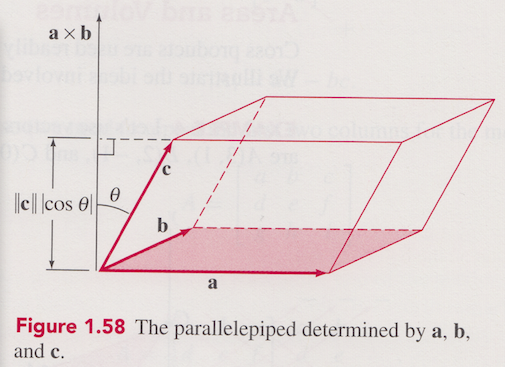
\includegraphics [scale=0.5] {ppd_volume.png} \end{center}

Recall that the direction of $\mathbf{a} \times \mathbf{b}$ is perpendicular to both vectors.   If we are careful to write the cross-product in the correct order using the right-hand rule, the result of the dot product will always be positive, with the projection of $\mathbf{c}$ onto the cross-product equal to the height of the solid.  In particular, for this arrangement, we must write $\mathbf{a} \times \mathbf{b}$, $\mathbf{b} \times \mathbf{c}$, or $\mathbf{c} \times \mathbf{a}$.

It doesn't matter which two vectors we choose as the base of our solid, the volume must come out the same.
\[ \mathbf{a} \cdot (\mathbf{b} \times \mathbf{c}) = \mathbf{b} \cdot (\mathbf{c} \times \mathbf{a}) = \mathbf{c} \cdot (\mathbf{a} \times \mathbf{b}) \]

\end{document}